\chapter{Algorytm weryfikacji}

Zastosowany algorytm weryfikacji modelowej opiera się głównie na \textit{on-the-fly OWCTY} \cite{Bar12}, który został dostosowany do wykorzystania w środowisku rozproszonym.

\begin{algorithm}
\caption{$ detectAcceptingCycle() $}
\label{alg:detectAcceptingCycle}
\begin{algorithmic}[1]
\REQUIRE $ G = (V,E,ACC) $

\STATE $ initialStates \leftarrow getInitialStates() $
\STATE $ approximationSet \leftarrow initialise(initialStates) $
\STATE $ oldSize \leftarrow \infty $
\WHILE{$ (approximationSet.size \neq oldSize)\ \mathbf{and}\ (approximationSet.size > 0) $}
  \STATE $ oldSize \leftarrow approximationSet.size $
  \STATE $ eliminateNoAccepting(approximationSet) $
  \STATE $ eliminateNoPredecessors(approximationSet) $
\ENDWHILE
\RETURN $ approximationSet.size > 0 $
\end{algorithmic}
\end{algorithm}

Algorytm OWCTY wykorzystuje sortowanie topologiczne dla detekcji cykli.
Zapewnia liniową złożoność czasową przy jednoczesnym uniknięciu przeszukiwania w głąb, co umożliwia wykonanie równoległe.
Niestety procedura sortowania topologicznego nie może bezpośrednio wykryć cykli akceptujących.
Zamiast tego wykorzystuje się eliminację cykli nieakceptujących.
Obliczany jest zbiór stanów poprzedzanych przez cykl akceptujący (\textit{approximationSet}).
Jeśli po zakończeniu algorytmu zbiór ten jest pusty, nie ma cyklu akceptującego.
Sam zbiór wylicza się w kilku fazach.
Pierwsza z nich, czyli \textit{initialise()} (algorytm \ref{alg:initialise}) eksploruje pełną przestrzeń stanów systemu oraz przygotowuje niezbędne dane dla kolejnych faz.
Kolejne dwie usuwają ze zbioru stany, które nie mogą być częścia cyklu akceptującego.

Jedna z nich to \textit{eliminateNoAccepting()} (algorytm \ref{alg:eliminateNoAccepting}).
Zaczyna się od pozostawienia w zbiorze jedynie stanów akceptujących (linie 3-10).
Następnie obliczane są wartości liczby poprzedników dla każdego wierzchołka.
To część procedury osiągalności, która poszerza cały zbiór, a ten może zawierać już nie tylko stany akceptujące (linie 11-22).

Ostatnia faza OWCTY to \textit{eliminateNoPredecessors()} (algorytm \ref{alg:eliminateNoPredecessors}).
Bazuje ona na sortowaniu topologicznym.
Wykorzystuje liczbę poprzedników wyliczonych w \textit{eliminateNoAccepting()}, aby iteracyjnie usuwać wierzchołki ze zbioru, kiedy ich stopień (w podgrafie tworzonym przez stany pozostałe w zbiorze) równy jest 0.
Kiedy wierzchołek znika ze zbioru, należy zmniejszyć stopień jego następników o 1.
Brak takich następników oznacza zakończenie fazy.
\textit{EliminateNoAccepting()} oraz \textit{eliminateNoPredecessors()} wykonywane są w pętli, dopóki zachodzą jakieś zmiany.

Opis użytych zmiennych/procedur w algorytmach \ref{alg:detectAcceptingCycle} i \ref{alg:initialise}:
\begin{itemize}
\item $ G = (V,E,ACC) $ - wejściowy graf składający się ze zbiorów wierzchołków, krawędzi i stanów akceptujących
\item \textit{getInitialStates()} - procedura zwracająca zbiór stanów początkowych dla grafu $G$
\item \textit{isAccepting(x)} - zwraca prawdę, jeśli stan $x$ jest akceptujący, fałsz w przeciwnym wypadku
\item \textit{acceptingCycleFound()} - służy do wcześniejszego zakończenia algorytmu (kiedy cykl akceptujący został wykryty bez eksploracji całej przestrzeni stanów)
\end{itemize}

% TODO opisac funkcje globalne: graf G=(V,E,ACC), getInitialStates(), isAccepting(x), acceptingCycleFound()

\begin{algorithm}
\caption{$ initialise(initialStates) $}
\label{alg:initialise}
\begin{algorithmic}[1]
\REQUIRE $ initialStates $

\STATE $ approximationSet \leftarrow initialStates $
\STATE $ q \leftarrow new\ Queue() $
\STATE $ q.pushBack(initialStates) $
\WHILE{$ q.isNotEmpty() $}
  \STATE $ s \leftarrow q.popFront() $
  \FORALL{$ t \in getSuccessors(s) $}
    \IF{$ t \notin approximationSet $}
      \STATE $ approximationSet.add(t) $
      \STATE $ q.pushBack(t) $
    \ENDIF
    \IF{$ isAccepting(t) $}
      \IF{$ (t == s)\ \mathbf{or}\ (approximationSet.getMap(s) == t) $}
        \STATE $ acceptingCycleFound() $
        \RETURN
      \ENDIF
      \STATE $ approximationSet.setMap(t, max(t, approximationSet.getMap(s))) $
    \ELSE
      \STATE $ approximationSet.setMap(t, approximationSet.getMap(s)) $
    \ENDIF
  \ENDFOR
\ENDWHILE
\RETURN $ approximationSet $
\end{algorithmic}
\end{algorithm}


\section{Heurystyka}

To zaaplikowanie heurystyki w fazie inicjalizacji (funkcja \textit{initialise()} w algorytmie \ref{alg:initialise}) modyfikuje oryginalny OWCTY.
Jedyna różnica to linie 11-19, które wykorzystują pomysł z algorytmu MAP.
Propaguje się jednego akceptującego poprzednika przez wszystkie nowo odkryte krawędzie.
Jeśli stan akceptujący zostanie przekazany do samego siebie, oznacza to wykrycie cyklu akceptującego, a obliczenia zostają przerwane (linia 13).
Zgodnie z działaniem algorytmu MAP, na stan akceptujący do rozpropagowania wybiera się ten maksymalny spośród stanów akceptujących odwiedzonych na ścieżce ze stanu początkowego do obecnego.

\begin{algorithm}
\caption{$ eliminateNoAccepting(approximationSet) $}
\label{alg:eliminateNoAccepting}
\begin{algorithmic}[1]
\REQUIRE $ approximationSet $

\STATE $ tmpApproximationSet \leftarrow \emptyset $
\STATE $ q \leftarrow new\ Queue() $
\FORALL{$ s \in approximationSet $}
  \IF{$ isAccepting(s) $}
    \STATE $ q.pushBack(s) $
    \STATE $ tmpApproximationSet.add(s) $
    \STATE $ tmpApproximationSet.setPredecessorCount(s,0) $
  \ENDIF
\ENDFOR
\STATE $ approximationSet \leftarrow tmpApproximationSet $
\WHILE{$ q.isNotEmpty() $}
  \STATE $ s \leftarrow q.popFront() $
  \FORALL{$ t \in getSuccessors(s) $}
    \IF{$ t \in approximationSet $}
      \STATE $ approximationSet.incrementPredecessorCount(t) $
    \ELSE
      \STATE $ q.pushBack(t) $
      \STATE $ approximationSet.add(t) $
      \STATE $ approximationSet.setPredecessorCount(t,0) $
    \ENDIF
  \ENDFOR
\ENDWHILE
\end{algorithmic}
\end{algorithm}

Faza inicjalizacji algorytmu OWCTY wymaga eksploracji całej przestrzeni stanów, więc została wykorzystana do wykonania detekcji cykli wykorzystując propagację maksymalnego akceptującego stanu.
W przeciwieństwie do alogrytmu MAP brakuje to repropagacji, aby złożoność obliczeniowa pozostała i liniowa i była proporcjonalna do rozmiaru grafu.
Skutek tego ograniczenia to brak wykrywalności wszystkich cykli (stąd to heurystyka).

\noindent
Wyróżnić można dwa podstawowe powody, kiedy metoda ta będzie nieskuteczna (pominie cykl):
\begin{enumerate}
  \item Maksymalny akceptujący poprzednik nie leży wewnętrz cyklu.
  \item Wartość maksymalnego akceptującego poprzednika nie wróci do źródła, mimo że cykl istnieje.
\end{enumerate}

\begin{algorithm}
\caption{$ eliminateNoPredecessors(approximationSet) $}
\label{alg:eliminateNoPredecessors}
\begin{algorithmic}[1]
\REQUIRE $ approximationSet $

\STATE $ q \leftarrow new\ Queue() $
\FORALL{$ s \in approximationSet $}
  \IF{$ approximationSet.getPredecessorCount(s) == 0 $}
    \STATE $ q.pushBack(s) $
  \ENDIF
\ENDFOR
\WHILE{$ q.isNotEmpty() $}
  \STATE $ s \leftarrow q.popFront() $
  \STATE $ approximationSet.remove(s) $
  \FORALL{$ t \in getSuccessors(s) $}
    \STATE $ approximationSet.decrementPredecessorCount(t) $
    \IF{$ approximationSet.getPredecessorCount(t) == 0 $}
      \STATE $ q.pushBack(t) $
    \ENDIF
  \ENDFOR
\ENDWHILE
\end{algorithmic}
\end{algorithm}

Pierwszy przypadek obsługiwany jest w oryginalnym algorytmie MAP poprzez iteracyjne usuwanie stanów akceptujących, co wymaga dodatkowej liczby przejść o liniowej złożoności. Drugi przypadek obsługuje repropagacja, która również nie mogła zostać zawarta ze względu na podniesienie złożoności obliczeniowej.

W sytuacji, gdy żadne z powyższych nie zachodzi, akceptujący cykl zostanie wykryty.
Przykłady z rys. \ref{fig:alg_heuristic_examples}:
\begin{enumerate}[label=(\alph*)]
\item Przypadek trywialny (jeden stan akceptujący). Wartość $B$ zostanie rozpropagowana do $C$ i $D$. W wyniku tego $B$ powróci do wezła źródłowego, więc cykl zostanie wykryty.
\item W tej sytuacji także nastąpi wykrycie cyklu, jednak po drodze występuje kilka stanów akceptujących. Ponieważ $ B > C \land B > D $, $B$ zostanie przesłane dalej.
\item Przypadek podobny do poprzedniego, lecz krawędź powrotna skierowana jest w $C$ (zamiast w $B$). Efekt tej zmiany to umiejscowienie największego akceptującego poprzednika poza cyklem ($ B > C \land B > D $). Taki cykl zostanie pominięty przez zastosowaną heurystykę (1. podstawowy powód).
\item Maksymalny akceptujący poprzednik znaduje się w cyklu, jednak to nie on go zaczyna. Próba propagacji wartości $C$ do $B$ zakończy się fiaskiem, ponieważ $ C < B $. Dalej $B$ przekazane zostanie do $B$. W wyniku tego porównuje się ze sobą obecną wartość $D$ ze stanem, do którego wraca krawędź. $ B \neq C $, więc do wykrycia cyklu nie dojdzie.
\end{enumerate}


\def \noderadius {1.2cm}
\def \noderadiuspt {0.6}
\def \radius {1.5}
\def \marginangle {30}
\begin{figure}
\centering

% w komentarzach wartosc MAP oryginalna i po algorytmie
% uda sie, wracamy do akceptujacego
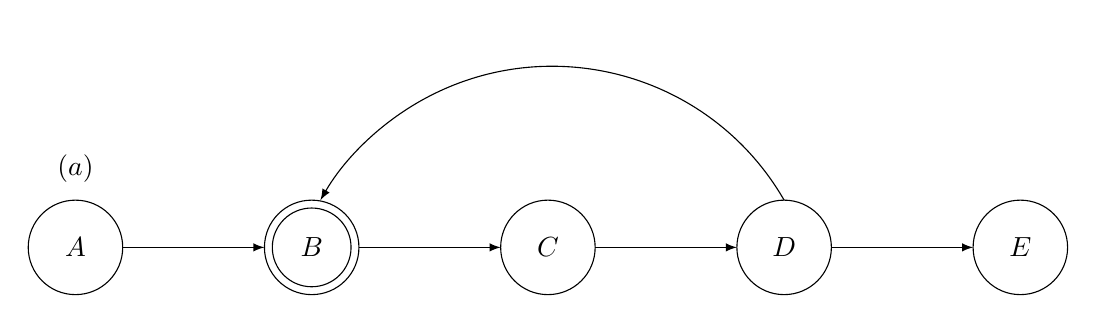
\begin{tikzpicture}
\node at (-4,1) {$ (a) $};
\draw (-4,0) node[draw, circle, minimum size=\noderadius] {$ A $}; % -/-
\draw[->, >=latex] (-4+\noderadiuspt,0) -- (-1-\noderadiuspt,0);
\draw (-1,0) node[draw, circle, minimum size=\noderadius] {$ B $}; % 5/5
\draw (-1,0) node[draw, circle, minimum size=\noderadius-0.2cm] {};
\draw[->, >=latex] (-1+\noderadiuspt,0) -- (2-\noderadiuspt,0);
\draw (2,0) node[draw, circle, minimum size=\noderadius] {$ C $}; % -/5
\draw[->, >=latex] (2+\noderadiuspt,0) -- (5-\noderadiuspt,0);
\draw (5,0) node[draw, circle, minimum size=\noderadius] {$ D $}; % -/5
\draw[->, >=latex] (5+\noderadiuspt,0) -- (8-\noderadiuspt,0);
\draw (8,0) node[draw, circle, minimum size=\noderadius] {$ E $}; % -/5
\draw[->, >=latex] (5,\noderadius/2) arc ({\marginangle}:{180 - \marginangle}:3.4);
\end{tikzpicture}

% uda sie, wartosc MAP ze stanu 2 przeszla na 3 i 4
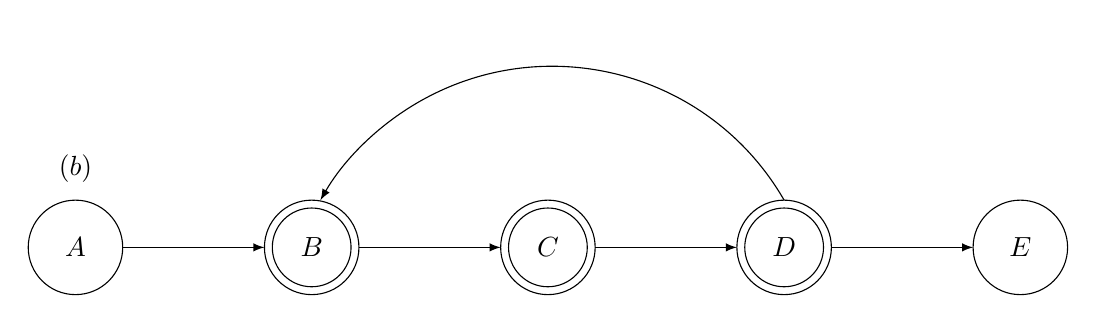
\begin{tikzpicture}
\node at (-4,1) {$ (b) $};
\draw (-4,0) node[draw, circle, minimum size=\noderadius] {$ A $}; % -/-
\draw[->, >=latex] (-4+\noderadiuspt,0) -- (-1-\noderadiuspt,0);
\draw (-1,0) node[draw, circle, minimum size=\noderadius] {$ B $}; % 5/5
\draw (-1,0) node[draw, circle, minimum size=\noderadius-0.2cm] {};
\draw[->, >=latex] (-1+\noderadiuspt,0) -- (2-\noderadiuspt,0);
\draw (2,0) node[draw, circle, minimum size=\noderadius] {$ C $}; % 4/5
\draw (2,0) node[draw, circle, minimum size=\noderadius-0.2cm] {};
\draw[->, >=latex] (2+\noderadiuspt,0) -- (5-\noderadiuspt,0);
\draw (5,0) node[draw, circle, minimum size=\noderadius] {$ D $}; % 3/5
\draw (5,0) node[draw, circle, minimum size=\noderadius-0.2cm] {};
\draw[->, >=latex] (5+\noderadiuspt,0) -- (8-\noderadiuspt,0);
\draw (8,0) node[draw, circle, minimum size=\noderadius] {$ E $}; % -/5
\draw[->, >=latex] (5,\noderadius/2) arc ({\marginangle}:{180 - \marginangle}:3.4);
\end{tikzpicture}

% nie uda sie -> mimo poprawnej pętli, stan 3 nie jest źródłem wartości propagowanej dalej (a)
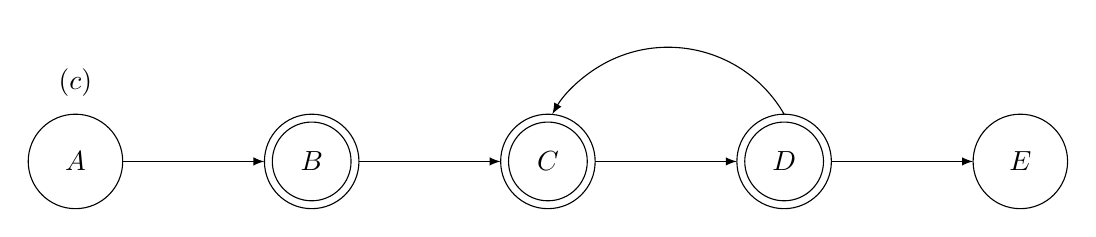
\begin{tikzpicture}
\node at (-4,1) {$ (c) $};
\draw (-4,0) node[draw, circle, minimum size=\noderadius] {$ A $}; % -/-
\draw[->, >=latex] (-4+\noderadiuspt,0) -- (-1-\noderadiuspt,0);
\draw (-1,0) node[draw, circle, minimum size=\noderadius] {$ B $}; % 5/5
\draw (-1,0) node[draw, circle, minimum size=\noderadius-0.2cm] {};
\draw[->, >=latex] (-1+\noderadiuspt,0) -- (2-\noderadiuspt,0);
\draw (2,0) node[draw, circle, minimum size=\noderadius] {$ C $}; % 4/5
\draw (2,0) node[draw, circle, minimum size=\noderadius-0.2cm] {};
\draw[->, >=latex] (2+\noderadiuspt,0) -- (5-\noderadiuspt,0);
\draw (5,0) node[draw, circle, minimum size=\noderadius] {$ D $}; % 3/5
\draw (5,0) node[draw, circle, minimum size=\noderadius-0.2cm] {};
\draw[->, >=latex] (5+\noderadiuspt,0) -- (8-\noderadiuspt,0);
\draw (8,0) node[draw, circle, minimum size=\noderadius] {$ E $}; % -/5
\draw[->, >=latex] (5,\noderadius/2) arc ({\marginangle}:{180 - \marginangle}:1.7);
\end{tikzpicture}

% nie uda się -> kolejne stany akceptujące mają wiekszą wartość MAP, przez co poprzednia zostaje zapomniana (c,b?)
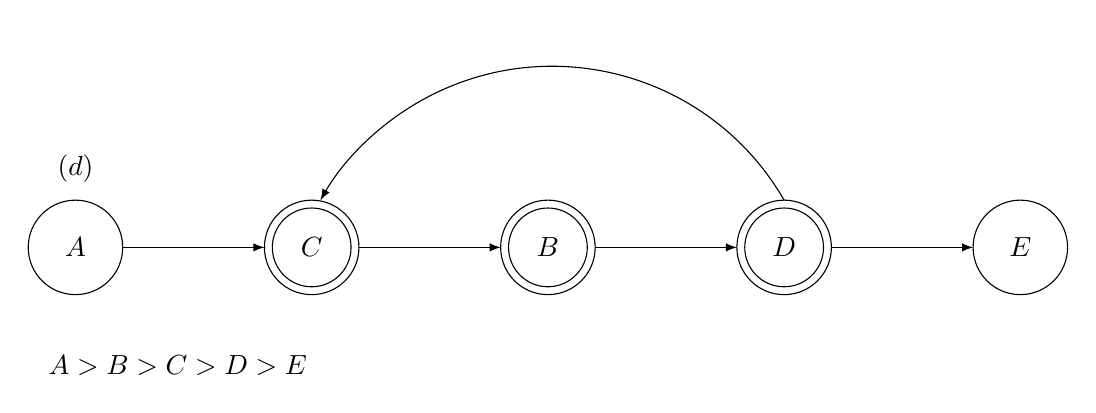
\begin{tikzpicture}
\node at (-4,1) {$ (d) $};
\draw (-4,0) node[draw, circle, minimum size=\noderadius] {$ A $}; % -/-
\draw[->, >=latex] (-4+\noderadiuspt,0) -- (-1-\noderadiuspt,0);
\draw (-1,0) node[draw, circle, minimum size=\noderadius] {$ C $}; % 5/5
\draw (-1,0) node[draw, circle, minimum size=\noderadius-0.2cm] {};
\draw[->, >=latex] (-1+\noderadiuspt,0) -- (2-\noderadiuspt,0);
\draw (2,0) node[draw, circle, minimum size=\noderadius] {$ B $}; % 6/6
\draw (2,0) node[draw, circle, minimum size=\noderadius-0.2cm] {};
\draw[->, >=latex] (2+\noderadiuspt,0) -- (5-\noderadiuspt,0);
\draw (5,0) node[draw, circle, minimum size=\noderadius] {$ D $}; % 3/6
\draw (5,0) node[draw, circle, minimum size=\noderadius-0.2cm] {};
\draw[->, >=latex] (5+\noderadiuspt,0) -- (8-\noderadiuspt,0);
\draw (8,0) node[draw, circle, minimum size=\noderadius] {$ E $}; % -/6
\draw[->, >=latex] (5,\noderadius/2) arc ({\marginangle}:{180 - \marginangle}:3.4);
\node at (-2.7,-1.5) {$ A > B > C > D > E $};
\end{tikzpicture}

\caption{Przykłady działania heurystyki algorytmu. W przypadkach (a) i (b) akceptujący cykl zostanie wykryty, jednak dla (c) i (d) już nie.}
\label{fig:alg_heuristic_examples}
\end{figure}


\section{Działanie w locie}

Działa on w locie poziomu 1.
W tym przypadku oznacza to, że może on zakończyć się przed eksploracją całego grafu stanów.
Powodem, przez który nie dzieje się tak zawsze, jest zastosowana heurystyka.
Pozwala ona wykryć część cykli akceptujących w locie, jednak są przypadki, kiedy nie wystarcza.
Wtedy cykl zostanie pominięty.
Do tego momentu algorytm ten okazuje się niewystarczający i może zwrócić niepoprawny wynik.
Zostało to uniknięte poprzez dodanie drugiej części, która odnajdzie już każdy cykl akceptujący.
Niestety nie działa ona w locie, więc potrzebuje wygenerowanej całej przestrzeni stanów.

\begin{figure}[h]
    \centering
    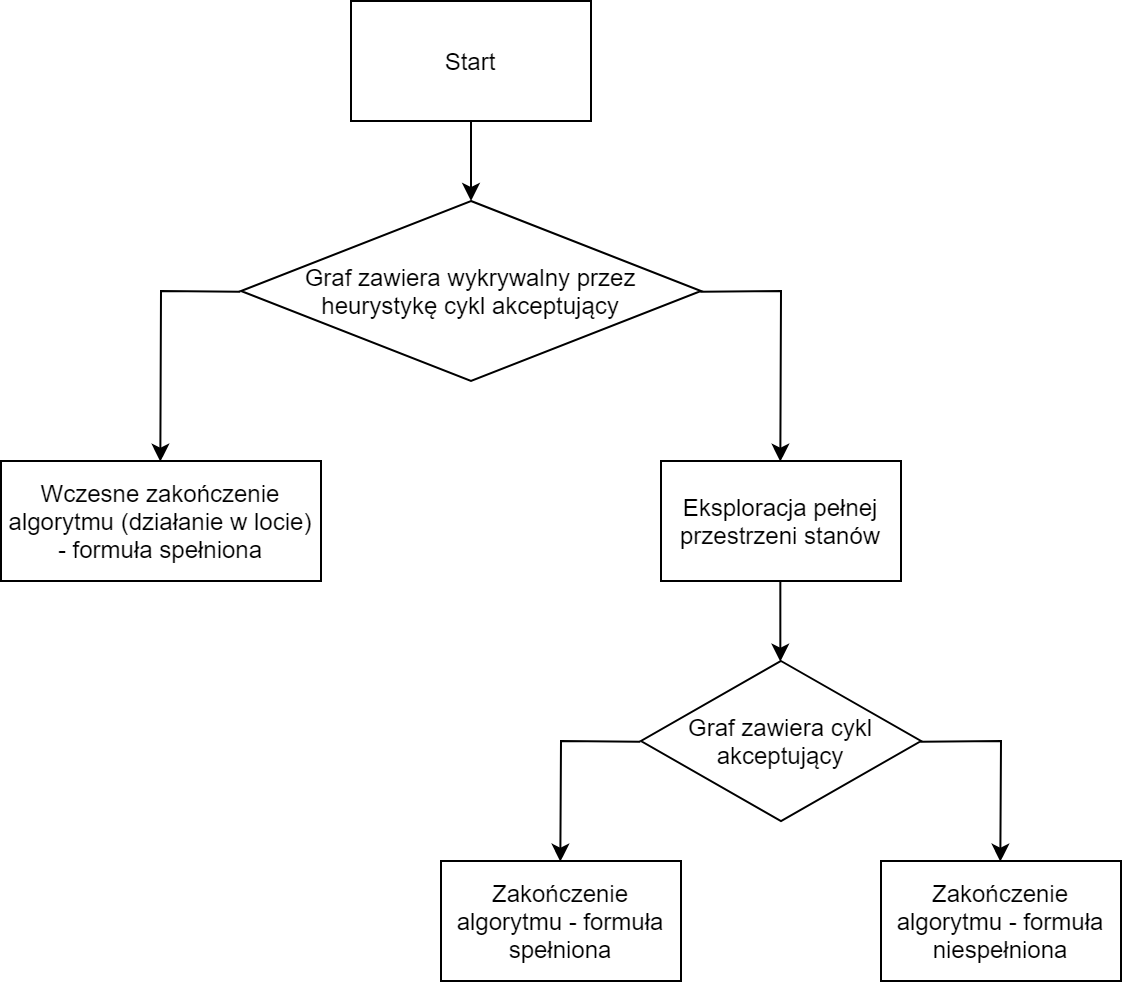
\includegraphics[height=11cm,keepaspectratio]{img/on-the-fly-diagram.png}
    \caption{Diagram przedstawiający kiedy dochodzi do wczesnego zakończenia algorytmu.}
    \label{fig:ltl_model_checking}
\end{figure}
